\documentclass[12pt]{article}
\usepackage[T1]{fontenc}
\usepackage[margin=2cm]{geometry}

\usepackage{amssymb}
\usepackage{amsmath}
\usepackage{tcolorbox}
\usepackage{xcolor}
\usepackage{framed}
\usepackage{euscript}
\usepackage{float}

\usepackage{verbatim}
\usepackage{mathrsfs}
\usepackage{graphicx}
\usepackage{multicol}

\usepackage{bbm,txfonts}
\usepackage{float}


\usepackage{titletoc}
\usepackage{tikz}
\usepackage{xspace}

\usepackage{enumitem}

\newcommand{\answer}{\vspace*{4pt} \noindent{\bf Solution: }}

\newcommand{\bb}[1]{\mathbb{#1}}
\renewcommand{\v}[1]{\boldsymbol{#1}}
\newcommand{\m}[1]{\mathbf{#1}}
\renewcommand{\c}[1]{\mathcal{#1}}
\usepackage{upquote}


\renewcommand{\tilde}{\widetilde}
\newcommand{\halmos}{\vspace{3mm} \hfill \mbox{$\Box$}}

\newcommand{\Var}{\mathbb{V}\mathrm{ar}}
\newcommand{\var}{\Var}

\newcommand{\Cov}{\mathbb{C}\mathrm{ov}}
\newcommand{\cov}{\Cov}

\renewcommand{\epsilon}{\varepsilon}
\renewcommand{\rho}{\varrho}
\renewcommand{\log}{\ln}
\renewcommand{\hat}{\widehat}

\newcommand{\iid}{\text{iid }}


% Bernoulli distribution
\newcommand{\Ber}{{\sf Ber}}
\newcommand{\ber}{\Ber}

% Binomial distribution
\newcommand{\Bin}{{\sf Bin}}
\newcommand{\bin}{\Bin}

% Cauchy distribution
\newcommand{\Cauchy}{{\sf Cauchy}}

% Negative binomial distribution
\newcommand{\NegBin}{{\sf NegBin}}

% Multinomial distribution
\newcommand{\Mnom}{{\sf Mnom}}
\newcommand{\mnom}{\Mnom}

% Geometric distribution
\newcommand{\Geo}{{\sf Geom}}
\newcommand{\geo}{\Geo}
\newcommand{\Geom}{\Geo}
\newcommand{\geom}{\Geo}
\newcommand{\G}{\Geo}

% Hypergeometric distribution
\newcommand{\Hyp}{{\sf Hyp}}

% Poisson distribution
\newcommand{\Poi}{{\sf Poi}}
\newcommand{\poi}{\Poi}
\newcommand{\Po}{\Poi}
\newcommand{\po}{\Poi}

% Uniform distribution (continuous)
\newcommand{\U}{\EuScript{U}}

% Exponential distribution
\newcommand{\Ex}{{\sf Exp}}
\newcommand{\ex}{\Ex}

% Normal / Gaussian distribution
\newcommand{\Nor}{\EuScript{N}}
\newcommand{\nor}{\Nor}

% Pareto distribution
\newcommand{\Pareto}{{\sf Pareto}}
\newcommand{\pareto}{\Pareto}

% Negative hypergeometric distribution
\newcommand{\NegHyp}{{\sf NegHyp}}

% Student's t distribution
\newcommand{\Student}{{\sf t}}
\newcommand{\student}{\Student}

% Gamma distribution
\newcommand{\Gam}{{\sf Gamma}}
\newcommand{\gam}{\Gam}

% Discrete uniform distribution
\newcommand{\DU}{{\sf DU}}

% Generic distribution
\newcommand{\Dist}{{\sf Dist}}

\newcommand{\Em}{{\mathbb E}}  % expectation
\newcommand{\Pm}{{\mathbb P}}  % probability measure
\newcommand{\R}{{\mathbb R}}

\newcommand{\gvn}{\,|\,}  % conditional (given)

\newcommand{\e}{\mathrm{e}} %Euler's e

\newcommand{\ds}{\displaystyle}

\newcommand{\di}{\mathrm{d}}  % use for differential symbol


\newcommand{\approxsim}{\stackrel{\mathrm{approx.}}{\sim}}

\newcommand{\iidsim}{\stackrel{\mathrm{iid}}{\sim}}
\newcommand{\simiid}{\iidsim}
\newcommand{\simiidt}{{\:{\sim}_{\mathrm{iid}}\:}}

%% Correlation
\newcommand{\Corr}{\mathrm{Corr}}
\newcommand{\corr}{\Corr}


\usepackage{cprotect}
\RequirePackage[formats]{listings}\RequirePackage{textcomp}

\lstnewenvironment{Pout}{%
  \lstset{backgroundcolor=\color{outcol},
  aboveskip= -2pt,  
  xleftmargin = 4pt,
  xrightmargin = 4pt,
  frame=single,
  upquote,
  framerule=1pt,
  basicstyle=\footnotesize\ttfamily,
  columns=fixed}}{}

%DK: See http://latexcolor.com/
\definecolor{applegreen}{rgb}{0.55, 0.41, 0.0}
\definecolor{gray1}{rgb}{0.98, 0.98, 0.98}
\definecolor{black}{rgb}{0, 0, 0}
\definecolor{cream}{rgb}{1.0, 0.99, 0.82}
\definecolor{islamicgreen}{rgb}{0.0, 0.56, 0.0}
\definecolor{vlgray}{gray}{0.9}
\definecolor{lgray}{gray}{0.7}
\definecolor{outcol}{gray}{0.9}

\tcbuselibrary{listings,skins,breakable,theorems}

\newenvironment{PC}{%
\tcblisting{breakable,listing only,colback=cream, enhanced, sharpish
corners,  boxrule=1pt,after, listing options =
   {language=Python,
  basicstyle=\footnotesize\ttfamily,        % the size of the fonts that are used for the code
  numbers=none,                   % where to put the line-numbers
%  numberstyle=\tiny\color{blue},  % the style that is used for the line-numbers
  xleftmargin=-10pt,
  aboveskip=-4pt,
  belowskip=-6pt,
  columns=fixed,
  basewidth=5pt,                     %separation of letters
%  stepnumber=1,                % the step between two line-numbers. If it's 1, each line will be numbered
%  numbersep=7pt,                  % how far the line-numbers are from the code
  backgroundcolor=\color{cream},  % choose the background color. You must add \usepackage{color}
  showspaces=false,               % show spaces adding particular underscores
  showstringspaces=false,         % underline spaces within strings
  showtabs=false,                 % show tabs within strings adding particular underscores
  %frame=single,                   % adds a frame around the code
  %frame=shadowbox,
  %rulecolor=\color{black},        % if not set, the frame-color may be changed on line-breaks within not-black text (e.g. comments (green here))
  tabsize=2,                     % sets default tabsize to 2 spaces
 % captionpos=b,                  % sets the caption-position to bottom
  breaklines=true,                % sets automatic line breaking
  breakatwhitespace=false,        % sets if automatic breaks should only happen at whitespace
  %title=\lstname,                 % show the filename of files included with \lstinputlisting;
                                  % also try caption instead of title
  keywordstyle=\color{blue},      % keyword style
  upquote,     % very important to get right quote for cut/paste
  commentstyle=\color{islamicgreen},   % comment style
  stringstyle=\color{red},      % string literal style
 % escapeinside={\%*}{*)},         % if you want to add a comment within your code
  morekeywords={*,...}
  			 }
    		}
    	}
{\endtcblisting}







\usepackage{fvextra}
\DefineVerbatimEnvironment{Code}{Verbatim}{
    fontsize=\footnotesize, % Adjust font size
    breaklines=true,        % Enable line wrapping
    breakanywhere=true      % Allow breaking anywhere
}

\begin{document}
\begin{center}

{\Large  {\bf MACHINE LEARNING (COMP7703)}

Assignment - Semester 1, 2025.

}
\end{center}

\vspace{20pt}

\textbf{1. Introduction}
\\
There are many different machine learning algorithms, and many metrics to evaluate them. In this assignment, we will focus on the K-Nearest Neighbour (K-NN) algorithm, Random Forest, and Deep Neural Networks, and the accuracy of each model. We will also looks at the different metrics to evaluate the performance of each model, and use these metrics to compare the suitability of each model for the given data.

\vspace{20pt}

\textbf{2. Aims}
\begin{itemize}
	\item To understand the K-Nearest Neighbour (K-NN) algorithm.
	\item To understand the accuracy of the K-NN classifier.
	\item To understand the effect of data imbalance on the accuracy of the K-NN classifier.
	\item To understand how to use cross-validation to improve the accuracy of the K-NN classifier.
\end{itemize}

\vspace{20pt}

\textbf{3. Data}
\\
The data used in this assignment is the \texttt{iris} dataset, which is a well-known dataset in the machine learning community. The dataset contains 150 data points, with 4 features and 3 classes. The features are the sepal length, sepal width, petal length, and petal width, and the classes are the species of iris flower: setosa, versicolor, and virginica. The dataset is available in the \texttt{sklearn} library.
\textbf{3.1 Data split}
\\
The data is split into three height categories: high, medium, and low. The data is split into 60\% training data, 20\% testing data, and 20\% validation data. The training data is used to train the each model, the testing data is used to test the accuracy of each model, and the validation data is used to compare the performance of the models. 

\vspace{20pt}

\textbf{3.2 Data imbalance}
\\
After splitting the data, there is an imbalance in the amount of training data assigned to each category in height. There are 17364 (29.73\%) data points in the high, 40800 (42.03\%) data points in the medium, and 27450 (28.23\%) in the low category. This is a significant imbalance, which is addressed by the use of Synthetic Minority Over-sampling Technique (SMOTE) to generate synthetic data points for the low category. The SMOTE algorithm generates synthetic data points by interpolating between existing data points in the low category. This is done by selecting a random data point from the low category, and then selecting a random data point from the k nearest neighbours of that data point. The synthetic data point is then generated by taking a weighted average of the two data points.

After applying SMOTE, the training data is balanced, with 24552 data points in each category.
 
\vspace{20pt}

\textbf{4. Principle Component Analysis}

To investigate the effect of dimensionality reduction on the accuracy of the models, we will use Principle Component Analysis (PCA) to reduce the dimensionality of the data. PCA is a linear transformation that transforms the data into a new coordinate system, where the first coordinate is the direction of maximum variance, the second coordinate is the direction of maximum variance orthogonal to the first coordinate, and so on. 

% Insert figure of Scree plot here
\begin{figure}[h!]
\centering
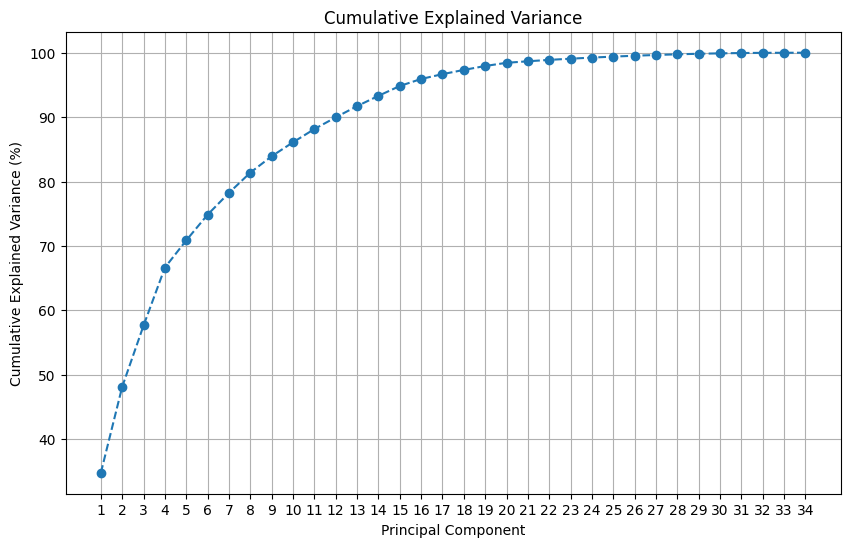
\includegraphics[width=0.8\textwidth]{figures/cum_var_scree.png}
\caption{Cumulative variance explained by each principal component.}
\label{fig:scree_plot}
\end{figure}

We see that approximately 95\% of the variance is explained by the top 16 principal components. This means that we can reduce the dimensionality of the data from 33 dimensions to 16 dimensions, while still retaining most of the information in the data. We will use dimensionality reduction in our models to in hopes of imporving accuracy and/or reducing computational expense.

\textbf{5. K-NN classifier}


\textbf{5.1 Accuracy of K-NN classifier}

\textbf{5.2 Cross-validation}

\textbf{6. Random Forest}

\textbf{7. Deep Neural Networks}

\end{document}
